\documentclass[article, 1.5space, letterpaper, 12pt, oneside, header, footer]{SydeClass}
\graphicspath{{images/}}
\usepackage{subfigure}
\usepackage{eqnarray}


% --------- Title Info -----------
\titlestyle{design} % used in SydeTitle.tex. Can equal one of the following values: design, work

\title{Lab 3}
\subtitle{Image Compression}

\coursecode{SYDE 475}
\department{Systems Design Engineering}

\author{Colin Heics, 20240543}
\authorheader{C. Heics}
\authortwo{Neil Sokol, 20265064}
\authorheadertwo{N. Sokol}

\date{\today}
\instructor{Alex Wong}

\subsectionfont{\normalsize}
\setcounter{secnumdepth}{2}
\setcounter{tocdepth}{1}

\input{matlabFormating}

% ############  ############
\begin{document}

% ---------- Title ------------
\input{SydeTitle}

% ############ Chapters ############
\pagenumbering{arabic}


\section{Overview}
The goal of this lab is to provide some hands-on experience with fundamental image enhancement and restoration concepts and techniques in both the spatial and frequency domain.

\subsubsection{Note}
This section has been included so that the section numbers match up with the original lab description.

\section{Chroma Subsampling}


\subsection{YCbCr channel decomposition}

\subsubsection{Describe the Cb and Cr channel images. Why do they appear this way?}
Cb is the blue difference chromatic component, and Cr is the red difference chromatic component.

\subsubsection{Compare the level of image detail in the Cb and Cr images with the Y channel image. Which contains more fine details? What does that say about the luma (Y) and chroma (Cb and Cr) channels?}

The Y channel contains the most fine image detail. This means that the majority of the high frequency components are found in the luma channel.

\begin{figure}[ht]
\centering
	\subfigure[Base Image]{
	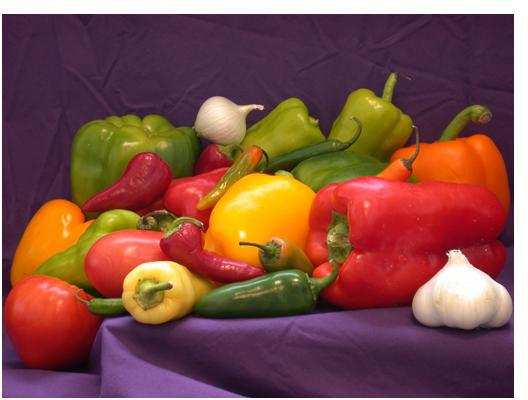
\includegraphics[width=0.45\linewidth]{question2/original_image}
	}
	\subfigure[Luma Component]{
	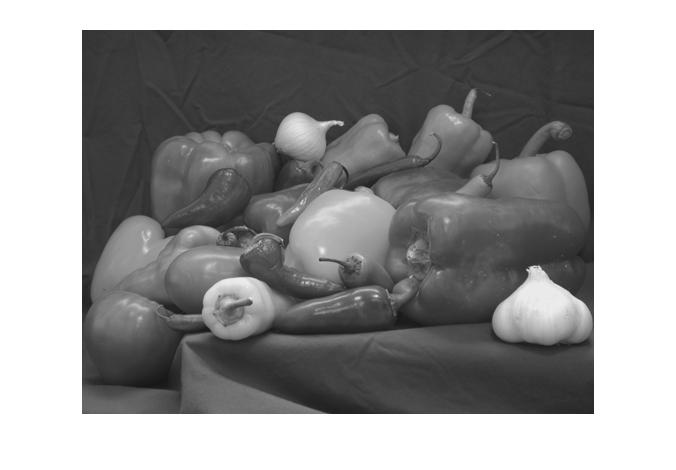
\includegraphics[width=0.45\linewidth]{question2/luma}
	}
	\subfigure[Cb Component]{
	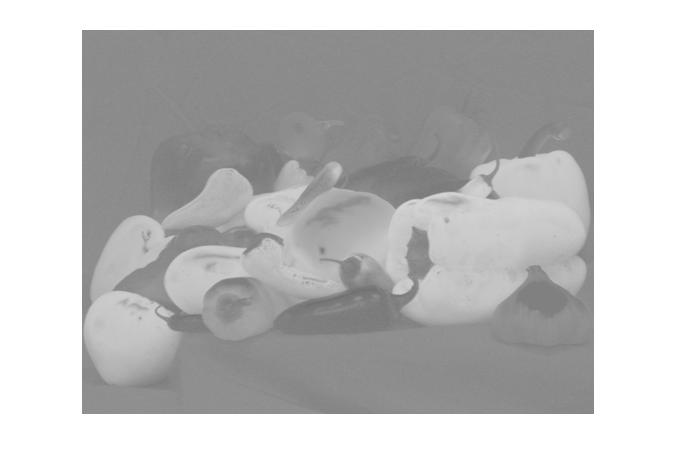
\includegraphics[width=0.45\linewidth]{question2/chroma_cb}
	}
	\subfigure[Cr Component]{
	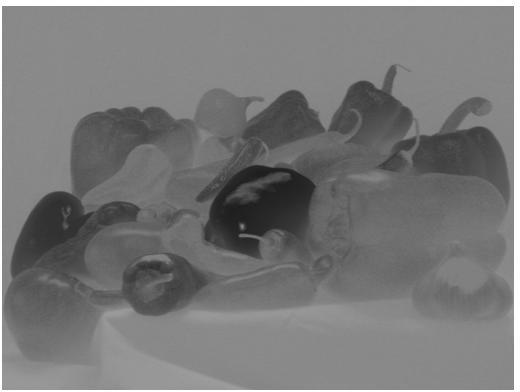
\includegraphics[width=0.45\linewidth]{question2/chroma_cr}
	}
	\caption{YCrCb channels of pepper image}
	\label{fig:noiseGeneration.toy}
\end{figure}	
	

\clearpage
\subsection{Chroma subsampling}
\subsubsection{Compare the resulting image from chroma sub-sampling with the original image. How large are the
visual differences}
The visual differences are essentially non-existant.

\begin{figure}[ht]
\centering	
	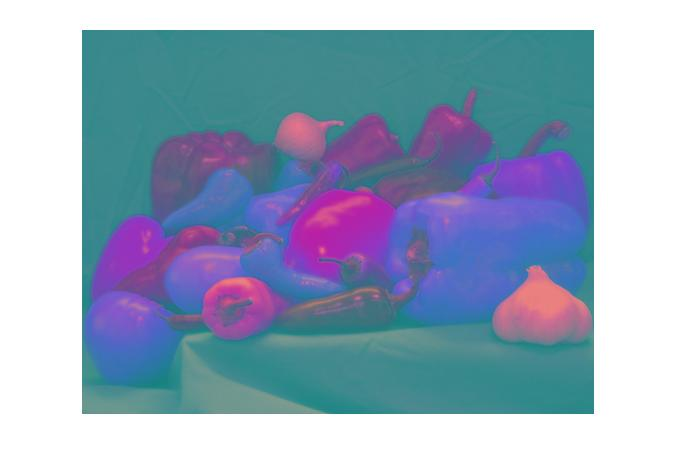
\includegraphics[width=0.65\linewidth]{question2/chroma_subsampled}
	\caption{Chroma subsampled image}
\end{figure}

\subsubsection{Based on the resulting image, what can you say about chroma sub-sampling and its effect on image
quality?}
Based on the subsampled images, it can be said that chroma sub-sampling has next to no impact on 

\clearpage
\subsection{Luma subsampling}
\subsubsection{Compare the resulting image from luma sub-sampling with the original image. How large are the
visual differences?}
The visual differences are more pronounced. The luma sub-sampled image is significantly blurrier than the original image.



\begin{figure}[ht]
\centering		
	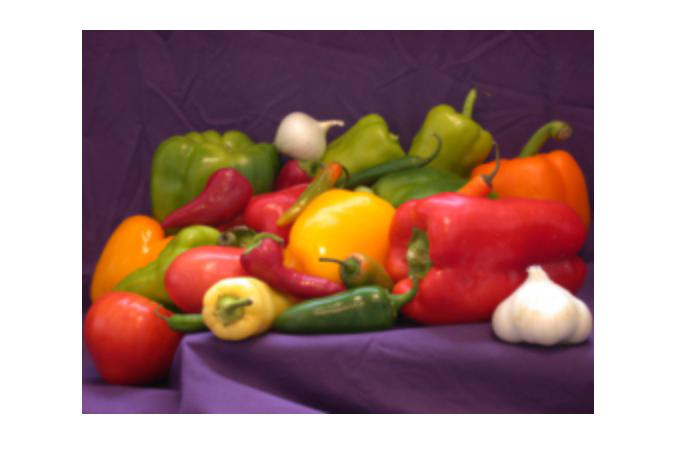
\includegraphics[width=0.65\linewidth]{question2/luma_subsampled}
	\caption{Luma subsampled image}
\end{figure}

\subsubsection{ Compare the resulting image from luma sub-sampling with the image produced using chroma subsampling. Which method performs better? Why}

\subsubsection{Based on the resulting image, what can you say about luma sub-sampling and its effect on image
quality}
\section{Image Transform}

\clearpage
\subsection{The discrete cosine transform matrix}

\subsubsection{What does each row of the DCT transform matrix represent? Look at the pattern for each row. If you still don't see it, try plotting each of the rows as a 1-D function.}
Each row of the DCT matrix is a cosine wave, with the period equal to $\frac{\pi}{n} \cdot (i-1)$; where $n$ is the number or rows in the DCT and $i$ is the row of the matrix being examined, with the exception of the first row is constant. The transform of the matrix is given by a product of a cosine oscilating in each direction.

\begin{table}[tbhc]
	\caption{Discrete Cosine Transform Matrix}
	\label{tbl:dctm}
	\begin{center}
		\begin{tabular}{ c | c | c | c | c | c | c | c}
0.3536	&	0.3536	&	0.3536	&	0.3536	&	0.3536	&	0.3536	&	0.3536	&	0.3536	\\
\hline
0.4904	&	0.4157	&	0.2778	&	0.0975	&	-0.0975	&	-0.2778	&	-0.4157	&	-0.4904	\\
\hline
0.4619	&	0.1913	&	-0.1913	&	-0.4619	&	-0.4619	&	-0.1913	&	0.1913	&	0.4619	\\
\hline
0.4157	&	-0.0975	&	-0.4904	&	-0.2778	&	0.2778	&	0.4904	&	0.0975	&	-0.4157	\\
\hline
0.3536	&	-0.3536	&	-0.3536	&	0.3536	&	0.3536	&	-0.3536	&	-0.3536	&	0.3536	\\
\hline
0.2778	&	-0.4904	&	0.0975	&	0.4157	&	-0.4157	&	-0.0975	&	0.4904	&	-0.2778	\\
\hline
0.1913	&	-0.4619	&	0.4619	&	-0.1913	&	-0.1913	&	0.4619	&	-0.4619	&	0.1913	\\
\hline
0.0975	&	-0.2778	&	0.4157	&	-0.4904	&	0.4904	&	-0.4157	&	0.2778	&	-0.0975	\\
		\end{tabular}
	\end{center}
\end{table}


\begin{figure}[ht]
\centering
	\subfigure[Heat map]{
	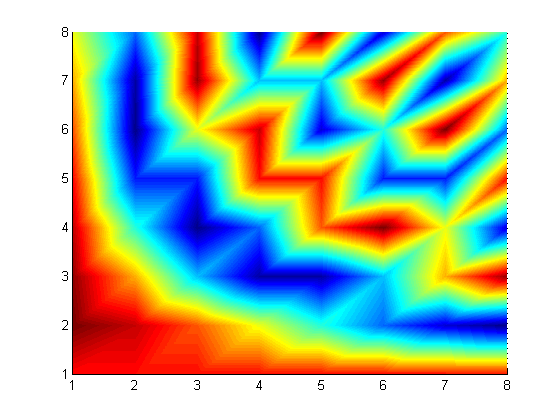
\includegraphics[width=0.45\linewidth]{question3/dctmtx_8_heat}
	}
	\subfigure[Rows of matrix]{
	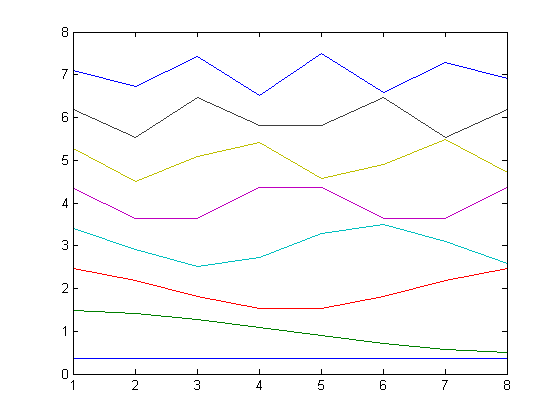
\includegraphics[width=0.45\linewidth]{question3/dctmtx_8_rows}
	}
\end{figure}


\clearpage
\subsection{Applying the discrete cosine transform matrix}



\begin{figure}[ht]
\centering
	\subfigure[Original image]{
	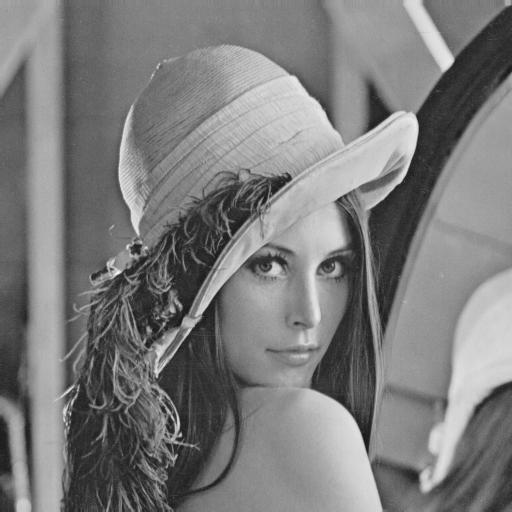
\includegraphics[width=0.45\linewidth]{question3/originalImage}
	}
	\subfigure[DCT 8 $\times$ 8 of original image]{
	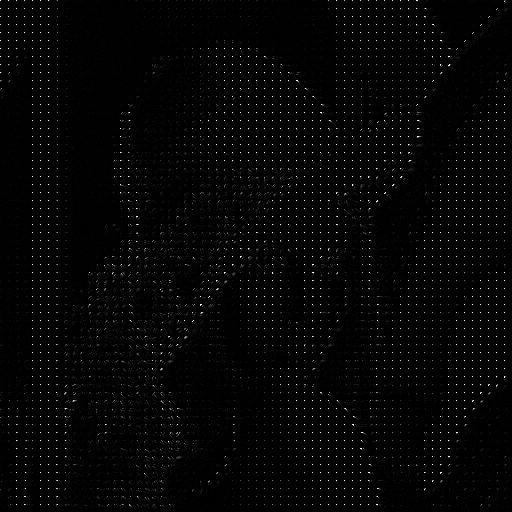
\includegraphics[width=0.45\linewidth]{question3/originalImage_dct}
	}
\end{figure}


\begin{figure}[ht]
\centering
	\subfigure[8 $\times$ 8 image block @ (297,81)]{
	
\includegraphics{question3/block1_8x8}
	}
	\subfigure[DCT]{
		\begin{tabular}{ c c c c c c c c}
		-136 &-31 & 2 &-6 &-1 &-6 &-1 &-4 \\
		14 &-6 & 5 &-6 & 3 &-4 & 2 &-1 \\
		-2 &-3 & 0 &-5 & 3 &-1 & 1 &-2 \\
		1 & 0 & 0 & 2 & 3 &-1 & 0 & 5 \\
		3 & 5 & 0 & 1 & 2 & 4 &-3 & 0 \\
		6 &-1 & 2 & 1 &-1 & 2 & 0 &-1 \\
		0 &-2 & 2 & 0 & 0 &-1 & 0 & 1 \\
		2 &-3 & 0 & 0 &-5 &-3 & 2 & 0 \\
		\\
		\end{tabular}
	}
\end{figure}

\begin{figure}[ht]
	\centering

	\subfigure[8 $\times$ 8 image block @ (1,1)]{
	
\includegraphics{question3/block2_8x8}
	}
	\subfigure[DCT]{
		\begin{tabular}{ c c c c c c c c}
		259 & 4 & 3 &-1 & 0 &-1 &-5 & 5 \\
		7 &-1 & 0 &-5 & 1 & 2 &-4 & 3 \\
		-6 &-1 &-2 & 1 &-1 &-1 & 1 &-3 \\
		2 & 1 & 1 & 0 &-1 &-2 & 0 & 1 \\
		-1 &-2 &-1 &-2 & 1 & 1 &-2 &-1 \\
		1 & 0 &-2 &-1 &-3 & 0 & 1 & 0 \\
		-2 & 0 & 3 & 1 & 1 &-3 &-2 &-1 \\
		1 &-1 &-3 &-2 &-1 & 1 & 0 & 0 \\
		\\
		\end{tabular}
	}
\end{figure}


\subsubsection{Describe the energy distribution of the DCT of the sub-images. What does each pixel represent? Explain why DCT would be useful for image compression in the context of the DCT energy distribution}

\subsubsection{Compare the DCT of the two sub-images. How are they different? Why? Explain in the context of the image characteristics at those locations and the DCT energy distribution}

\subsection{Compressing the DCT image by discarding high-frequency data}

\subsubsection{Describe how the reconstructed image looks compared to the original image. Why does it look this way?}

\subsubsection{What artifact is most prominent in the image? Why does this artifact appear?}

\subsubsection{What conclusions can you draw about the DCT in terms of image compression? Does it work well? If yes, why does it work well?}
\section{Quantization}

\subsection{Quantization with the 8 $\times$ 8 JPEG standard}

\begin{table}[tbhc]
	\caption{JPEG standard 8 $\times$ 8}
	\label{tbl:dctm}
	\begin{center}
		\begin{tabular}{ c c c c c c c c}
16 & 11 & 10 & 16 & 24 & 40 & 51 & 61 \\
12 & 12 & 14 & 19 & 26 & 58 & 60 & 55 \\
14 & 13 & 16 & 24 & 40 & 57 & 69 & 56 \\
14 & 17 & 22 & 29 & 51 & 87 & 80 & 62 \\
18 & 22 & 37 & 56 & 68 & 109 & 103 & 77 \\
24 & 35 & 55 & 64 & 81 & 104 & 113 & 92 \\
49 & 64 & 78 & 87 & 103 & 121 & 120 & 101 \\
72 & 92 & 95 & 98 & 112 & 100 & 103 & 99 \\
		\end{tabular}
	\end{center}
\end{table}



\subsubsection{What happens to the DCT coeffcients when quantization is performed? What effect does it have on image quality?}

When quantization is peformed, the coefficients of the DCT tend towards zero due to rounding. The coefficients in the upper left hand corner of the DCT, representing low frequency image information, maintain a non-zero value.

Quantization reduces the information in high frequency regions of each block. This reduces high frequency detail in a local area. However, since the transform is performed on a block, some overall structure is maintained in the neghborhood of the pixel, allowing the image to still maintain high apparent sharpness.

As the pixels are no longer near their original values, this approach fares poorly when measured acording the PSNR. However, the subjective quality and sharpness of the image is quite good.

\subsubsection{Compare the reconstructed image produced using 3Z with the original image. Why does the reconstructed image look this way?}

The image in 3Z contains slight blocking and banding artifacts, most visible on Lena's arm. This blocky appearance is due to the reduction in high frequency components in each block. When taken to the extreme, each block will approximate it's DC value, but at lower values it will reduce the number of intensities produce a slight blocking look to the image.

\subsubsection{Compare the reconstructed images produced by the different levels of quantization, as well as the PSNR for each reconstructed image. What happens as the level of quantization increases?}

As the level of quantization increases, the image appears to have more banding in areas of gradation and also displays prominent blocking artifacts.

The PSNR of the image is drastically decreased, as many pixels are far from their original values, spiking the MSE of the image.

Perceptually, each image maintains the structure of the image, and when squinting or viewing the image zoomed out, the images appear very similar.

\subsubsection{Which artifact becomes more prominent as the level of quantization increase? Why?}

Blocking artifacts become very prominent as the level of quantization increases. As quantization increases, all values except the DC value of the DCT approach zero. This causes a block that may have once contained detail to assume the average value of the pizels contained within the block.

\subsubsection{What conclusions can you draw about the quantization process? Explain in the context of the trade-off between compression performance and image quality.}

The quantization process can reduce the number of distinct values within a 8 $\times$ 8 DCT block from 64 to much less (~4-10), which drastically reduces the number of values that must be stored. The lower number of distinct values can dramtically improve the performance of run length encoding.

Since a much lower number of intensity values are stored, this can introduce undesirable image artifacts such as banding and blocking. When compressing an image with JPEG compression, a large reduction in distinct image values can be obtained with a small loss in perceptual image quality. For example image Z1 appears very similar to the original image (despite the PSNR value). Examining a single DCT block @ (201,201) the block contains only 13 non-zero DCT coefficients compared to 64 for the original image, a large reduction in size.

\begin{figure}[ht]
\centering
	\subfigure[JPEG Z1; PSNR +11.63dB]{
	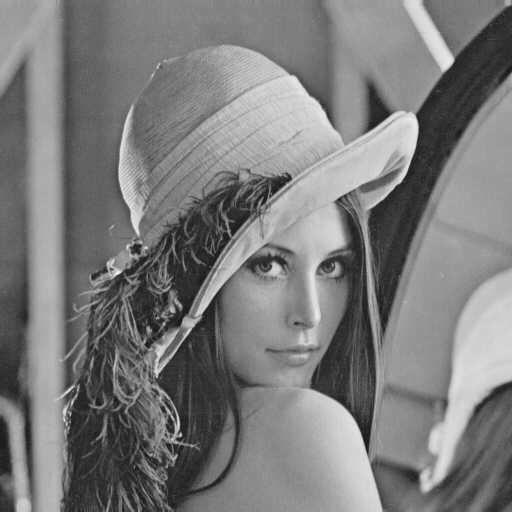
\includegraphics[width=0.45\linewidth]{question4/jpeg_Z1}
	}
	\subfigure[JPEG Z3; PSNR +8.22dB]{
	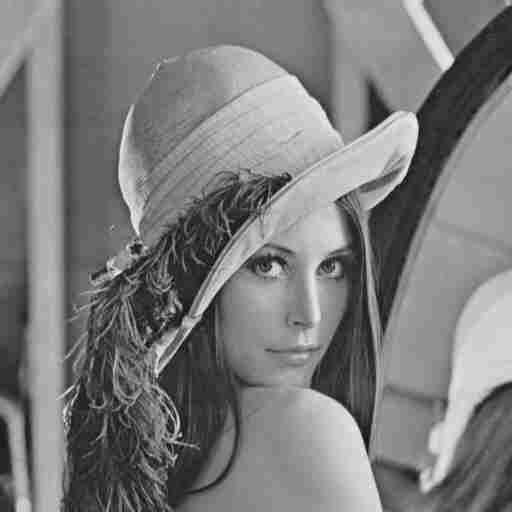
\includegraphics[width=0.45\linewidth]{question4/jpeg_Z3}
	}
	\subfigure[JPEG Z5; PSNR +6.31dB]{
	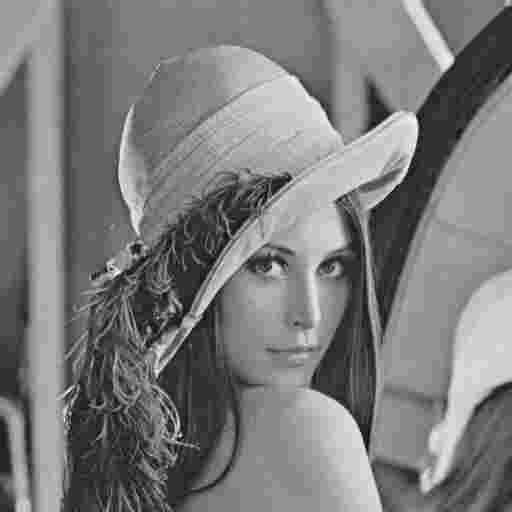
\includegraphics[width=0.45\linewidth]{question4/jpeg_Z5}
	}
	\subfigure[JPEG Z1; PSNR +3.25dB]{
	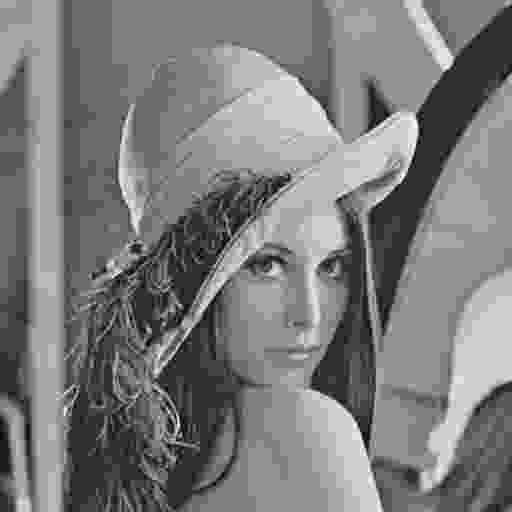
\includegraphics[width=0.45\linewidth]{question4/jpeg_Z10}
	}

\end{figure}




\appendix
\newpage

\section{Matlab Code}
\subsection{PSNR function}
\lstinputlisting[language=Matlab]{"matlabFiles/psnr.m"}

\subsection{Chroma Subsampling}
\lstinputlisting[language=Matlab]{"matlabFiles/lab3_q2.m"}

\subsection{Image Transform}
\lstinputlisting[language=Matlab]{"matlabFiles/lab3_q3.m"}

\subsection{Quantization}
\lstinputlisting[language=Matlab]{"matlabFiles/lab3_q2.m"}















% -------- Bibliography --------
%\addcontentsline{toc}{chapter}{\hspace{13pt} References}
\bibliography{refs}

\end{document}  